\documentclass[border=8pt]{standalone}
\usepackage{amsmath}
\usepackage{tikz}
\usetikzlibrary{arrows.meta,positioning,calc,decorations.pathreplacing}
\begin{document}
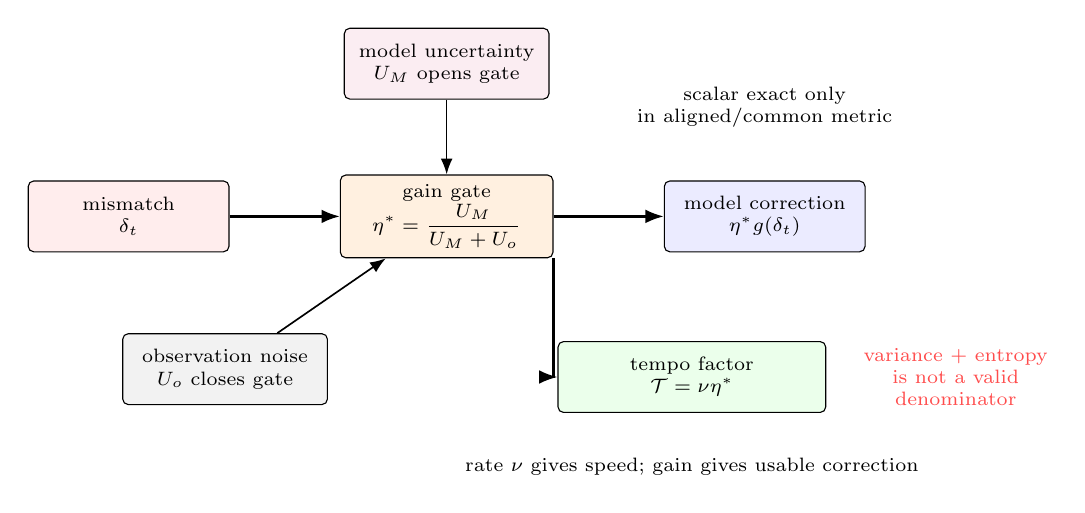
\begin{tikzpicture}[
  box/.style={draw, rounded corners=2pt, align=center, minimum width=2.55cm, minimum height=0.9cm, font=\scriptsize},
  gate/.style={draw, rounded corners=2pt, align=center, minimum width=2.7cm, minimum height=1.05cm, font=\scriptsize, fill=orange!12},
  note/.style={align=center, font=\scriptsize},
  arr/.style={-Latex, thick},
  thinarr/.style={-Latex, semithick}
]

\node[box, fill=red!7] (delta) {mismatch\\$\delta_t$};
\node[gate, right=1.4cm of delta] (gain) {gain gate\\$\eta^\ast=\dfrac{U_M}{U_M+U_o}$};
\node[box, fill=blue!8, right=1.4cm of gain] (update) {model correction\\$\eta^\ast g(\delta_t)$};

\draw[arr] (delta) -- (gain);
\draw[arr] (gain) -- (update);

\node[box, fill=purple!7, above=0.95cm of gain, minimum width=2.6cm] (um) {model uncertainty\\$U_M$ opens gate};
\node[box, fill=gray!10, below left=0.95cm and 0.15cm of gain, minimum width=2.6cm] (uo) {observation noise\\$U_o$ closes gate};
\draw[thinarr] (um) -- (gain);
\draw[thinarr] (uo) -- (gain);

\node[note, above=0.55cm of update] {scalar exact only\\in aligned/common metric};

\node[box, fill=green!8, below right=1.05cm and 0.05cm of gain, minimum width=3.4cm] (tempo) {tempo factor\\$\mathcal T=\nu\eta^\ast$};
\draw[arr] (gain.south east) |- (tempo.west);

\node[note, right=0.35cm of tempo, text=red!70] {variance + entropy\\is not a valid\\denominator};
\node[note, below=0.45cm of tempo] {rate $\nu$ gives speed; gain gives usable correction};

\end{tikzpicture}
\end{document}
